\documentclass[11pt]{article}

\usepackage[utf8]{inputenc}
\usepackage[margin=1in]{geometry}  % Adjust page margins
\usepackage{graphicx}              % For including images (PDF, PNG, JPG)
\usepackage[inkscapelatex=false]{svg}
\usepackage{listings}              % For including code
\usepackage{xcolor}                % For custom colors
\usepackage{hyperref}              % For hyperlinks in the PDF
\usepackage{amsmath, amssymb, amsthm} % For math symbols and environments
\usepackage{mathrsfs}
\usepackage{enumitem}
\geometry{a4paper, margin=1in} % Set margin to 1 inch
\usepackage{fancyhdr} % For header and footer
\usepackage{hyperref} % For clickable links in the PDF
\usepackage{array} % For table column formatting
\usepackage{times} % Uses Times font for the text
\usepackage{float}
\usepackage{multirow}
\usepackage{booktabs}


\title{CMOR 421/521 Assignment 4: Using CUDA to implement Matrix Multiplication and Matrix Transpose.}
\author{Yuhao Liu}
\date{\today}

% --------------------------------------------------------------------------------
% Customize the appearance of code listings (for C++ syntax).
% --------------------------------------------------------------------------------
\lstdefinestyle{C++Style}{
    language=C++,
    basicstyle=\small\ttfamily,
    keywordstyle=\color{blue}\bfseries,
    commentstyle=\color{gray},
    stringstyle=\color{magenta},
    numbers=left,
    numberstyle=\tiny,
    stepnumber=1,
    breaklines=true,
    tabsize=4,
    showstringspaces=false
}

% If you store SVG images in a subfolder, specify the path here. 
% e.g.: \svgpath{{../images/}}
\svgpath{{./}}

\begin{document}

\maketitle

\tableofcontents
\bigskip

\newpage

\section{Directory structure}
Below is my file organization for this assignment. 
My final zip file follows this structure ( \texttt{docs/} for LaTeX, \texttt{src/} for source files, and \texttt{include/} for header files):

\begin{figure}[H]
    \centering
    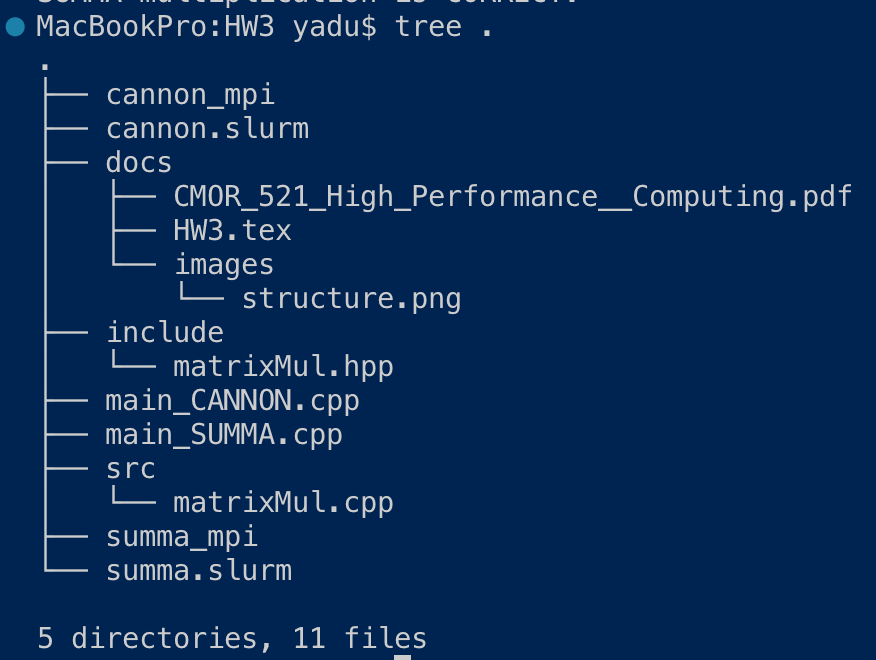
\includegraphics[width=0.5\linewidth]{Assignments/HW3/docs/images/structure.png}
    \caption{structure}
    \label{fig:structure}
\end{figure}

\begin{itemize}
    \item The \verb|include| folder and \verb|src| folder have \verb|matrixMul.hpp| and \verb|matrixMul.cpp|. In \verb|matrixMul.cpp|, there are 2 help function 
    \begin{itemize}
        \item \texttt{void testMul(const int N, double* serialC, double* mpiC);}  
    
        \item \texttt{void serialMatMult(const int N, double* C, const double* A, const double* B);}  
    \end{itemize}

    \item The \verb|main_CANNON.cpp| and \verb|main_SUMMA.cpp| contain the Cannon's algorithm and SUMMA algorithm respectively.
    \item The \verb|cannon_mpi| and \verb|summa_mpi| are executable files. Both of them already complied by \verb|-O3| optimization flag.
    \item The \verb|cannon.slurm| and \verb|summa.slurm| are sbatch scripts.
\end{itemize}

\newpage

\section{How to build and run}
All code should run in NOTS.
\subsection{Request interative session}
\begin{verbatim}
    srun --pty --partition=commons --reservation=cmor421 --ntasks=1
    --cpus-per-task=1 --gres=gpu --mem=5G --time=00:30:00 $SHELL
\end{verbatim}

\subsection{Build and run matrix multiplication}
\begin{verbatim}
    nvcc matmul.cu
    nvprof ./a.out <Matrix size> <Version for Matrix Multiplication>
    nvprof --metrics flop_count_sp,dram_read_transactions,dram_write_transactions ./a.out <Matrix size> <Version for Matrix Multiplication>

\end{verbatim}
where \verb|<Version for Matrix Multiplication>| is \verb|1, 2, 3|. E.g., 
\begin{verbatim}
    nvprof ./a.out 2048 1
\end{verbatim}
    
In this case you will run the the version 1 of matrix multiplication with $2048 \times 2048$ matrix. In addition, you can directly run my \verb|slurm| script with
\begin{verbatim}
    sbatch matmul.slurm
\end{verbatim}

\subsection{Build and run matrix transpose}
\begin{verbatim}
    nvcc matTranspose.cu
    nvprof ./a.out <Matrix size>
    nvprof --metrics gld_throughput,gst_throughput ./a.out <Matrix size>

\end{verbatim}
E.g., 
\begin{verbatim}
    nvprof ./a.out 2048
\end{verbatim}
In this case you will run both of naive matrix transpose and blocking, shared memory matrix transpose with $2048 \times 2048$ matrix. In addition, you can directly run my \verb|slurm| script with
\begin{verbatim}
    sbatch matTranspose.slurm
\end{verbatim}

\newpage

\section{Results}
All results are obtained from NOTS and the GPU I used is \verb|NVIDIA Tesla V100-PCIE-32GB|

\subsection{Matrix multiplication}
The results for Matrix Multiplication can be found in file \verb|matmul_BLOCKSIZE16/32.txt|.
\subsubsection{Run time}
\begin{table}[H]
\centering
\begin{tabular}{|c|c|c|c|c|c|}
\hline
\textbf{Kernel}   & \boldmath$N$\unboldmath & \textbf{BLOCKSIZE} & \textbf{Avg time (ms)} & \textbf{Min time (ms)} & \textbf{Max time (ms)} \\ \hline
matmul\_v1        & 2048  & 16  & 47.013  & 47.013  & 47.013  \\
matmul\_v2        & 2048  & 16  & 9.2806  & 9.2806  & 9.2806  \\
matmul\_v3        & 2048  & 16  & 5.1794  & 5.1794  & 5.1794  \\ \hline
matmul\_v1        & 4096  & 16  & 333.92  & 333.92  & 333.92  \\
matmul\_v2        & 4096  & 16  & 65.313  & 65.313  & 65.313  \\
matmul\_v3        & 4096  & 16  & 37.128  & 37.128  & 37.128  \\ \hline
\end{tabular}
\caption{Profiling results for CUDA matrix multiplication (BLOCKSIZE=16) at $N=2048$ and $N=4096$.}
\label{tab:matmul_combined_updated}
\end{table}

\begin{table}[H]
\centering
\begin{tabular}{|c|c|c|c|c|c|}
\hline
Kernel      & $N$   & BLOCKSIZE & Avg Time (ms) & Min Time (ms) & Max Time (ms) \\ \hline
matmul\_v1  & 2048  & 32        & 91.050        & 91.050        & 91.050        \\
matmul\_v2  & 2048  & 32        & 8.0414        & 8.0414        & 8.0414        \\
matmul\_v3  & 2048  & 32        & 4.6569        & 4.6569        & 4.6569        \\ \hline
matmul\_v1  & 4096  & 32        & 644.07        & 644.07        & 644.07        \\
matmul\_v2  & 4096  & 32        & 65.174        & 65.174        & 65.174        \\
matmul\_v3  & 4096  & 32        & 37.046        & 37.046        & 37.046        \\ \hline
\end{tabular}
\caption{Profiling results for CUDA matrix multiplication (BLOCKSIZE=32) at $N=2048$ and $N=4096$.}
\label{tab:matmul_combined}
\end{table}


\subsubsection{GFLOPS/sec}
\verb|GFLOPS/sec| is defined as: 
\[
\text{GFLOPS/sec} = \frac{\text{Total Floating Point Operations (FLOP)}}{\text{Excution time (in seonds)} \times 10^9}
\]
where:
\begin{itemize}
    \item \texttt{flop\_count\_sp} = Total number of floating point operations (single precision)
    \item \texttt{Avg Times} = Excution time (in seonds)
\end{itemize}
Finally, the \verb|GFLOPS/sec| calculation formula is:

\[
\text{GFLOPS/sec} = \frac{\text{flop\_count\_sp}}{32 \times (\text{Avg kernal time} \times 10^9)
}
\]

The following table is the \verb|GFLOPS/sec| results when $N = 2048, 4096$ and \verb|BLOCKSSIZE = 16| with different version of matrix multiplication.

\begin{table}[H]
\centering
\begin{tabular}{|c|c|c|c|}
\hline
\textbf{Kernel}   & \boldmath$N$\unboldmath & \textbf{Avg time (ms)} & \textbf{GFLOPS/sec} \\ \hline
matmul\_v1        & 2048  & 47.013   & 365.43  \\ 
matmul\_v2        & 2048  & 9.2806   & 1851.17 \\ 
matmul\_v3        & 2048  & 5.1794   & 3316.99 \\ \hline
matmul\_v1        & 4096  & 333.92   & 411.60  \\ 
matmul\_v2        & 4096  & 65.313   & 2104.33 \\ 
matmul\_v3        & 4096  & 37.128   & 3701.79 \\ \hline
\end{tabular}
\caption{Combined GFLOPS performance for $N=2048$ and $N=4096$.}
\label{tab:matmul_gflops_updated}
\end{table}

The following table is the \verb|GFLOPS/sec| results when $N = 2048, 4096$ and \verb|BLOCKSSIZE = 32| with different version of matrix multiplication.

\begin{table}[H]
\centering
\begin{tabular}{|c|c|c|c|}
\hline
\textbf{Kernel}   & \boldmath$N$\unboldmath & \textbf{Avg time (ms)} & \textbf{GFLOPS/sec} \\ \hline
matmul\_v1        & 2048  & 91.046  & 188.76  \\ 
matmul\_v2        & 2048  & 8.0433  & 2137.85 \\ 
matmul\_v3        & 2048  & 6.8625  & 2503.72 \\ \hline
matmul\_v1        & 4096  & 644.04  & 213.42  \\ 
matmul\_v2        & 4096  & 65.394  & 2102.89 \\ 
matmul\_v3        & 4096  & 54.372  & 2528.09 \\ \hline
\end{tabular}
\caption{Profiling results (Avg kernel time and GFLOPS/sec) for $N=2048$ and $N=4096$}
\label{tab:matmul_gflops_combined}
\end{table}



\subsubsection{Arithmetic intensity}
Arithmetic Intensity (AI) is defined as:

\[
\text{Arithmetic Intensity} = \frac{\text{Total Floating Point Operations (FLOP)}}{\text{Total Bytes Transferred to/from DRAM}}
\]

where:

\begin{itemize}
    \item \texttt{flop\_count\_sp} = Total number of floating point operations (single precision)
    \item \texttt{dram\_read\_transactions} = Number of DRAM read transactions
    \item \texttt{dram\_write\_transactions} = Number of DRAM write transactions
    \item Each transaction typically transfers \textbf{32 bytes} (because it involves single-precision \texttt{float}, usually corresponding to a 32-byte cache line)
\end{itemize}

Thus, the total DRAM transferred data volume is:

\[
\text{Total Bytes} = 32 \times (\text{dram\_read\_transactions} + \text{dram\_write\_transactions})
\]

Finally, the AI calculation formula is:

\[
\text{AI} = \frac{\text{flop\_count\_sp}}{32 \times (\text{dram\_read\_transactions} + \text{dram\_write\_transactions})
}
\]

The following table is the arithmetic intensity results when $N = 2048, 4096$ and \verb|BLOCKSSIZE = 32| with different version of matrix multiplication.
\begin{table}[H]
\centering
\resizebox{\textwidth}{!}{
\begin{tabular}{|c|c|c|c|c|c|c|}
\hline
\textbf{Kernel}   & \boldmath$N$\unboldmath & \textbf{BLOCKSIZE} & \textbf{flop\_count\_sp}              & \textbf{dram\_read\_transactions} & \textbf{dram\_write\_transactions} & \textbf{AI (FLOP/byte)} \\ \hline
matmul\_v1        & 2048  & 16 & $1.7180\times10^{10}$ & 54\,620\,046       & 857\,863        & 9.68  \\ 
matmul\_v2        & 2048  & 16 & $1.7180\times10^{10}$ & 53\,988\,032       & 624\,804        & 9.83  \\ 
matmul\_v3        & 2048  & 16 & $1.7180\times10^{10}$ & 64\,511\,202       & 756\,200        & 8.23  \\ \hline
matmul\_v1        & 4096  & 16 & $1.3744\times10^{11}$ & 591\,602\,704      & 3\,242\,460      & 7.22  \\ 
matmul\_v2        & 4096  & 16 & $1.3744\times10^{11}$ & 270\,670\,070      & 2\,199\,450      & 15.74 \\ 
matmul\_v3        & 4096  & 16 & $1.3744\times10^{11}$ & 270\,483\,950      & 2\,366\,130      & 15.74 \\ \hline
\end{tabular}
}
\caption{Combined Profiling and Arithmetic Intensity (AI) for $N=2048$ and $N=4096$.}
\label{tab:AI_combined_updated}
\end{table}


The following table is the arithmetic intensity results when $N = 2048, 4096$ and \verb|BLOCKSSIZE = 32| with different version of matrix multiplication.
\begin{table}[H]
\centering
\resizebox{\textwidth}{!}{
\begin{tabular}{|c|c|c|c|c|c|c|}
\hline
\textbf{Kernel}   & \boldmath$N$\unboldmath & \textbf{BLOCKSIZE} & \textbf{flop\_count\_sp}              & \textbf{dram\_read\_transactions} & \textbf{dram\_write\_transactions} & \textbf{AI (FLOP/byte)} \\ \hline
matmul\_v1        & 2048   & 32       & $1.7180\times10^{10}$ & 14\,305\,192       & 764\,601        & 35.63                   \\ 
matmul\_v2        & 2048   & 32       & $1.7180\times10^{10}$ & 15\,854\,944       & 621\,818        & 32.58                   \\ 
matmul\_v3        & 2048   & 32       & $1.7180\times10^{10}$ & 16\,020\,134       & 694\,805        & 32.12                   \\ \hline
matmul\_v1        & 4096   & 32       & $1.3744\times10^{11}$ & 272\,109\,225      & 2\,779\,070      & 15.62                   \\ 
matmul\_v2        & 4096   & 32       & $1.3744\times10^{11}$ & 271\,233\,134      & 2\,200\,003      & 15.71                   \\ 
matmul\_v3        & 4096   & 32       & $1.3744\times10^{11}$ & 270\,714\,581      & 2\,349\,926      & 15.73                   \\ \hline
\end{tabular}
}
\caption{Combined Profiling and Arithmetic Intensity (AI) for $N=2048$ and $N=4096$.}
\label{tab:AI_combined}
\end{table}

\newpage

\subsection{Matrix transpose}
The results for Matrix Multiplication can be found in file \verb|matTranspose_BLOCKSIZE16/32.txt|.

\subsubsection{Run time}

\begin{table}[H]
\centering
\begin{tabular}{|l|c|c|c|c|c|}
\hline
\textbf{Kernel}                             & \boldmath$N$\unboldmath & \textbf{BLOCKSIZE} & \textbf{Avg time (ms)} & \textbf{Min time (ms)} & \textbf{Max time (ms)} \\ \hline
Naive matrix transpose                      & 2048  & 16  & 0.19798  & 0.19798  & 0.19798  \\
Shared‐memory matrix transpose              & 2048  & 16  & 0.097247 & 0.097247 & 0.097247 \\ \hline
Naive matrix transpose                      & 4096  & 16  & 0.88121  & 0.88121  & 0.88121  \\
Shared‐memory matrix transpose              & 4096  & 16  & 0.35488  & 0.35488  & 0.35488  \\ \hline
\end{tabular}
\caption{Profiling results for CUDA matrix transpose (BLOCKSIZE=16) at $N=2048$ and $N=4096$.}
\label{tab:matTranspose_combined_updated}
\end{table}

\begin{table}[H]
\centering
\begin{tabular}{|l|c|c|c|c|c|}
\hline
\textbf{Kernel}                             & \boldmath$N$\unboldmath & \textbf{BLOCKSIZE} & \textbf{Avg time (ms)} & \textbf{Min time (ms)} & \textbf{Max time (ms)} \\ \hline
Naive matrix transpose                      & 2048  & 32  & 1.2107   & 1.2107   & 1.2107   \\
Shared-memory matrix transpose              & 2048  & 32  & 0.052672 & 0.052672 & 0.052672 \\ \hline
Naive matrix transpose                      & 4096  & 32  & 6.4144   & 6.4144   & 6.4144   \\
Shared-memory matrix transpose              & 4096  & 32  & 0.18723  & 0.18723  & 0.18723  \\ \hline
\end{tabular}
\caption{Profiling results for CUDA matrix transpose (BLOCKSIZE=32) at $N=2048$ and $N=4096$.}
\label{tab:matTranspose_combined_updated}
\end{table}

\subsubsection{GB/s}
\begin{table}[H]
\centering
\resizebox{\textwidth}{!}{
\begin{tabular}{|l|c|c|c|c|}
\hline
\textbf{Kernel}                             & \textbf{BLOCKSIZE} & \textbf{global load (GB/s)} & \textbf{global store (GB/s)} & \textbf{combined (GB/s)} \\ \hline
Naive matrix transpose (2048)               & 16                 & 78.82                        & 630.59                       & 709.41                   \\
Shared‐memory matrix transpose (2048)       & 16                 & 154.65                       & 154.65                       & 309.30                   \\ \hline
Naive matrix transpose (4096)               & 16                 & 70.53                        & 564.27                       & 634.80                   \\
Shared‐memory matrix transpose (4096)       & 16                 & 182.60                       & 182.60                       & 365.20                   \\ \hline
\end{tabular}
}
\caption{Global (device) memory throughput for CUDA matrix transpose at $N=2048$ and $N=4096$.}
\label{tab:matTranspose_bw_nvprof}
\end{table}

\begin{table}[H]
\centering
\resizebox{\textwidth}{!}{
\begin{tabular}{|l|c|c|c|c|}
\hline
\textbf{Kernel}                             & \textbf{BLOCKSIZE} & \textbf{global load (GB/s)} & \textbf{global store (GB/s)} & \textbf{combined (GB/s)} \\ \hline
Naive matrix transpose (2048)               & 32                 & 13.627                       & 109.01                       & 122.64                   \\
Shared-memory matrix transpose (2048)       & 32                 & 300.24                       & 300.24                       & 600.48                   \\ \hline
Naive matrix transpose (4096)               & 32                 & 9.6832                       & 77.466                       & 87.1492                  \\
Shared-memory matrix transpose (4096)       & 32                 & 327.12                       & 327.12                       & 654.24                   \\ \hline
\end{tabular}
}
\caption{Global (device) memory throughput for CUDA matrix transpose at $N=2048$ and $N=4096$.}
\label{tab:matTranspose_bw_nvprof}
\end{table}

\end{document}